% Boyang Wang
% Nov. 19, 2018 
% boyang.wang@uc.edu
% CS 5058/6158 Data Security and Privacy
% This is an ACM template for the final project

\documentclass[sigconf]{acmart}

\settopmatter{printacmref=false}
\setcopyright{none}
\acmConference[]{}{}{}
\acmDOI{}
\acmISBN{}
\acmPrice{}
\settopmatter{printfolios=true}

\usepackage{booktabs} % For formal tables

% additional packages by Boyang
\usepackage{graphicx}
\usepackage{array}
\usepackage{amsmath}
\usepackage[ruled, vlined, linesnumbered]{algorithm2e}
\usepackage{algorithmic}
\let\Bbbk\relax
\usepackage{amssymb} %\varnothing
\usepackage{framed,multicol} 
\usepackage{subfigure}

\usepackage[framemethod=TikZ]{mdframed}
%\mdfsetup{frametitlealignment=\center}

%\renewcommand{\algorithmicrequire}{\textbf{Input:}}
%\renewcommand{\algorithmicensure}{\textbf{Output:}}

% Copyright
%\setcopyright{none}
%\setcopyright{acmcopyright}
%\setcopyright{acmlicensed}
\setcopyright{rightsretained}
%\setcopyright{usgov}
%\setcopyright{usgovmixed}
%\setcopyright{cagov}
%\setcopyright{cagovmixed}


% DOI
\acmDOI{10.475/123_4}

% ISBN
\acmISBN{123-4567-24-567/08/06}

%Conference
\acmConference[ACM XXXXX'18]{ACM XXXXX}{XX 2018}{XX, XX, XX} 
\acmYear{2018}
\copyrightyear{2018}

\acmPrice{15.00}


\begin{document}
\title{Analysis of 'When Malware is Packin' Heat; Limits of Machine Learning Classifiers Based on Static Analysis Features'}
%\titlenote{Produces the permission block, and
%  copyright information}
%\subtitle{This is a Draft}
%\subtitlenote{The full version of the author's guide is available as
%  \texttt{acmart.pdf} document}


\author{Thomas Turner}
\affiliation{%
  \institution{M14507785}
}

\author{Nathan Hafely}
\affiliation{%
  \institution{enter M number here} 
}

%\author{G.K.M. Tobin}
%\authornote{The secretary disavows any knowledge of this author's actions.}
%\affiliation{%
%  \institution{Institute for Clarity in Documentation}
%  \streetaddress{P.O. Box 1212}
%  \city{Dublin} 
%  \state{Ohio} 
%  \postcode{43017-6221}
%}
%\email{webmaster@marysville-ohio.com}

% The default list of authors is too long for headers}
\renewcommand{\shortauthors}{B. Wang et al.}


% \begin{abstract}
% To maintain search functionalities without losing data privacy on untrusted remote servers, e.g., public clouds, many Searchable Encryption (SE) schemes have been proposed to search over encrypted data without decryption. Normally, a SE scheme leaks access pattern by default in order to provide correct search results to users. Unfortunately, by utilizing access pattern, some recent attacks, such as \textit{range injection attacks}, can easily recover the plaintexts of encrypted data through a set of injected range queries. 
% \end{abstract}

%
% The code below should be generated by the tool at
% http://dl.acm.org/ccs.cfm
% Please copy and paste the code instead of the example below. 
%
\begin{CCSXML}
<ccs2012>
 <concept>
  <concept_id>10010520.10010553.10010562</concept_id>
  <concept_desc>Computer systems organization~Embedded systems</concept_desc>
  <concept_significance>500</concept_significance>
 </concept>
 <concept>
  <concept_id>10010520.10010575.10010755</concept_id>
  <concept_desc>Computer systems organization~Redundancy</concept_desc>
  <concept_significance>300</concept_significance>
 </concept>
 <concept>
  <concept_id>10010520.10010553.10010554</concept_id>
  <concept_desc>Computer systems organization~Robotics</concept_desc>
  <concept_significance>100</concept_significance>
 </concept>
 <concept>
  <concept_id>10003033.10003083.10003095</concept_id>
  <concept_desc>Networks~Network reliability</concept_desc>
  <concept_significance>100</concept_significance>
 </concept>
</ccs2012>  
\end{CCSXML}

%\ccsdesc[500]{Computer systems organization~Embedded systems}
%\ccsdesc[300]{Computer systems organization~Redundancy}
%\ccsdesc{Computer systems organization~Robotics}
%\ccsdesc[100]{Networks~Network reliability}

%\keywords{ACM proceedings, \LaTeX, text tagging}


\maketitle

% Introduction Section
\section{Introduction}
\label{sec:intro}

With the rise of machine learning and artificual intelligence in recent years, many malware analysis experts have begun to research how these new tools can be used in their field. Many papers have begun to be published on the topic of using machine learning classifiers to distinguish between packed benign and packed malicious samples. The paper that we analyzed aims to verify the accuracy of these tests and see for themselves if machine learning can indeed be used to distinguish the maliciousness of packed samples based on static features alone \cite{Aghakhani2020}. 

Creating tools to automatically detect if a sample is malicious or not is very sought after in the malware field. Currently the best and most effective way to determine if a sample is malicious is to have an expert analyzing it using various static and dynamic analysis tools. This process entails placing the malware in an isolated environment and analyuzing the static features such as imports, strings, and assembly code without running the code. Then the analyst will run debug the code to see any registry key changes, file system changes, or network connections the sample is attempting to make. This process can be very tedious and can take an expert a long time to complete.

There are also many online tools now such as VirusTotal that be used to automatically scan a sample to determine if it is malicious or not. But, this method also has many downsides. VirusTotal works by using signature-based detection methods to determine if a sample is malicious. So, if the signature of a sample is similar to a known malware, then VirusTotal will detect that the given sample is potentially malicious \cite{Aghakhani2020}. This technique is effective at detecting previosuly known malware, but will struggle on types of malware that it has never encoutnered before. 

VirusTotal is also known to struggle with packed samples. The paper mentions a study that was conducted by Lakshaman Nataraj. In this study, they collected a large number of benign Windows executables and then packed them with with four different common packers. Next, they submitted all of these samples to VirusTotal. From this experiemnt, they found that 96.7 percent of the samples caused ten or more malicious detections on VirusTotal \cite{Aghakhani2020}. This shows that VirusTotal also uses packing as a strong indicator of malciousness instead of the actual functionality of a sample. 

Nowadays, many benign samples are also packed to protect the authors from getting their intellectual property stole \cite{Aghakhani2020}. Therefore, it is no longer the normal for exclusively malicious samples to be packed. Figure 1 below shows the results of a brief experiment that the researchers conducted. In this experiemnt, they collected a large number of samples from the real world and then analyzed them to see how many of them were packed based on each cateogry of benign, malicious, and suspicious \cite{Aghakhani2020}. The results show that in the worst quarters around 50\% of the benign samples that they collected were packed \cite{Aghakhani2020}. 
\begin{figure}[htbp]
    \centering
    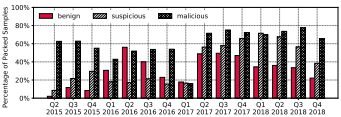
\includegraphics[width=0.5\textwidth]{benign_and_malicious_prevalence.png}
    \caption{Prevalence of packed samples in the wild.}
    \label{fig:packing}
\end{figure}

Through their experiments, the researchers show that packing routines do perserve some information on the function and maliciousness of a sample, but it is not enough to be applied to packers and packing routines that the classifier has never seen. Additionally, the classifier is susceptible to adversarial attacks \cite{Aghakhani2020}. This means that if malware authors can place benign code in their malware to try and confuse the classifier into thinking that the entire program is benign. 

% System/Threat Model
\section{System/Threat Model}
\label{sec:system}

For their experiments, the researchers used samples exclusiuvely from the Windows x86 operating system. The samples can be broken up into four unique categories: unpacked benign, packed benign, unpacked malicious, and packed malicious \cite{Aghakhani2020}. For each individual experiment, the data was broken up into a training set and a testing set. The type of classiifer that was used for the analysis was a random forest model. Additionally, the classifier was trained on nine different sets of features in the samples (PE Headers, PE Sections, DLL Imports, API Imports, Rich Header, Byte n-grams, Opcode n-grams, Strings, File Generic) \cite{Aghakhani2020}. 

% Methodology
\section{Methodology}
\label{sec:methodology}

This is the Methodology Section.

% Experiment Results and Analysis
\section{Experiment Results and Analysis}
\label{sec:results}

This is the Experiment Results and Analysis Section.

% Conclusioon and Discussion
\section{Conclusion and Discussion}
\label{sec:conclusion}

This is the Conclusion and Discussion Section. 

\bibliographystyle{ACM-Reference-Format}
\bibliography{main} 
%\bibliography{sample-bibliography} 

\newpage

%\input{appendix}

\end{document}
